\documentclass[11pt, letterpaper]{article}

% Mandatory Packages
\usepackage{amsmath}
\usepackage{amssymb}
\usepackage{amsthm}
\usepackage{geometry}
\usepackage{tikz}
\usetikzlibrary{arrows.meta, positioning, shapes, backgrounds}
\usepackage{mathrsfs}
\usepackage{mathtools}
\usepackage{hyperref}
\usepackage{enumitem}
\usepackage{tcolorbox}

% Page Geometry
\geometry{
    top=1in,
    bottom=1in,
    left=1in,
    right=1in
}

% Theorem Environments
\newtheorem{theorem}{Theorem}[section]
\newtheorem{lemma}[theorem]{Lemma}
\newtheorem{proposition}[theorem]{Proposition}
\newtheorem{corollary}[theorem]{Corollary}
\newtheorem{definition}[theorem]{Definition}
\newtheorem{axiom}[theorem]{Axiom}

\theoremstyle{remark}
\newtheorem*{remark}{Remark}
\newtheorem*{heuristic}{Heuristic}

% Custom Commands
\newcommand{\R}{\mathbb{R}}
\newcommand{\Z}{\mathbb{Z}}
\newcommand{\N}{\mathbb{N}}
\newcommand{\Q}{\mathbb{Q}}
\newcommand{\E}{\mathbb{E}}
\newcommand{\Prob}{\mathbb{P}}
\newcommand{\F}{\mathcal{F}}
\newcommand{\simlog}{\sim}

% Title Information
\title{\textbf{Homework Chapter 5: Existence and Proof by Contradiction}}
\author{Tashfeen Omran}
\date{September 2026}

\begin{document}

\maketitle
\tableofcontents
\newpage

% ==========================================
% PART 1: Introduction, Context, and Prerequisites
% ==========================================
\section{Part 1: Comprehensive Introduction, Context, and Prerequisites}

\subsection{Core Concepts \& Axioms}
In the rigorous study of abstract mathematics, establishing the truth or falsehood of a proposition requires formal logical frameworks. This chapter focuses on two foundational techniques: \textbf{Counterexamples} and \textbf{Proof by Contradiction}. 

A universally quantified statement takes the form $\forall x \in S, P(x)$, meaning ``for all elements $x$ in the set $S$, the property $P(x)$ holds.'' To disprove such a statement, one must prove its logical negation: $\sim (\forall x \in S, P(x))$. By the rules of first-order logic, this is equivalent to $\exists x \in S, \sim P(x)$. The specific element $x$ that satisfies $\sim P(x)$ is called a \textbf{counterexample}.

When direct proof is intractable, we employ \textbf{Proof by Contradiction} (Reductio ad Absurdum). To prove a proposition $R$, we assume its negation, $\sim R$, is true. Through valid logical deductions, we arrive at a contradiction, denoted as $C \land \sim C$ (a statement that is simultaneously true and false). By the \textit{Law of Non-Contradiction}, this is impossible. Therefore, our initial assumption $\sim R$ must be false, forcing $R$ to be true.

\subsection{Intuition and Set-Theoretic Foundations}
Imagine a probability space $(\Omega, \F, \Prob)$. Proving a universal statement is akin to showing that an event $A$ occurs almost surely, i.e., $\Prob(A) = 1$. Finding a counterexample is equivalent to identifying a specific outcome $\omega \in \Omega$ such that $\omega \notin A$, thereby proving $\Prob(A) < 1$ (or $A \neq \Omega$ in a strict set-theoretic sense). 

Proof by contradiction operates on the \textit{Law of Excluded Middle} ($P \lor \sim P$). If we partition our logical space into two mutually exclusive and exhaustive sets (the universe where $R$ is true, and the universe where $R$ is false), and we demonstrate that the universe where $R$ is false collapses into logical impossibility (an empty set $\emptyset$), we are left with only one valid reality: $R$ must be true.

\subsection{Historical Context and Motivation}
The method of contradiction dates back to ancient Greek mathematics. The most famous historical application was by the Pythagoreans (specifically attributed to Hippasus of Metapontum) in the 5th century BCE. They believed all numbers were rational (commensurable). However, when applying the Pythagorean theorem to a right isosceles triangle with leg lengths of $1$, they discovered the hypotenuse $\sqrt{2}$. By assuming $\sqrt{2}$ was rational, they derived a contradiction regarding the parity of integers, shattering the Pythagorean worldview and birthing the study of irrational numbers and real analysis.

\subsection{Key Theorems, Lemmas, and Formulas}
\begin{itemize}
    \item \textbf{Negation of Universal Quantifier:} $\sim (\forall x \in S, P(x)) \equiv \exists x \in S, \sim P(x)$.
    \item \textbf{Negation of Implication:} $\sim (P \implies Q) \equiv P \land \sim Q$.
    \item \textbf{Law of Non-Contradiction:} $\sim (P \land \sim P)$ is a tautology.
    \item \textbf{Principle of Explosion (Ex Falso Quodlibet):} $(P \land \sim P) \implies Q$. From a contradiction, any statement follows.
    \item \textbf{Parity Definitions:} An integer $n$ is even if $\exists k \in \Z$ such that $n = 2k$. It is odd if $\exists k \in \Z$ such that $n = 2k + 1$.
    \item \textbf{Rationality:} A real number $x$ is rational ($x \in \Q$) if $\exists p, q \in \Z$ with $q \neq 0$ such that $x = \frac{p}{q}$.
\end{itemize}

\subsection{Prerequisites}
To master this chapter, the reader must be fluent in:
\begin{enumerate}
    \item \textbf{First-Order Logic:} Manipulating quantifiers ($\forall, \exists$) and logical connectives ($\land, \lor, \implies, \sim$).
    \item \textbf{Basic Number Theory:} Divisibility rules, modular arithmetic, and the fundamental theorem of arithmetic.
    \item \textbf{Algebraic Manipulation:} Expanding polynomials, factoring, and working with inequalities.
\end{enumerate}

\newpage
% ==========================================
% PART 2: Detailed Homework Solutions
% ==========================================
\section{Part 2: Detailed Homework Solutions (Rigorous Proofs)}

\subsection{Section 5.1: Counterexamples}

\textbf{Exercise 5.1.} Disprove the statement: If $a$ and $b$ are any two real numbers, then $\log(ab) = \log(a) + \log(b)$.
\begin{proof}
To disprove the universal statement $\forall a, b \in \R, \log(ab) = \log(a) + \log(b)$, we must find a counterexample: a specific pair $a, b \in \R$ such that the premise is true (they are real numbers) but the conclusion is false or undefined.
Let $a = -1$ and $b = -1$. Both $a, b \in \R$.
Evaluate the left-hand side (LHS):
\[ \log(ab) = \log((-1)(-1)) = \log(1) = 0 \]
Evaluate the right-hand side (RHS):
\[ \log(a) + \log(b) = \log(-1) + \log(-1) \]
In the domain of real numbers, the logarithm function $\log(x)$ is strictly defined for $x > 0$. Therefore, $\log(-1)$ is undefined in $\R$.
Since the LHS evaluates to $0$ and the RHS is undefined, the equality $\log(ab) = \log(a) + \log(b)$ fails. Thus, $a = -1, b = -1$ serves as a counterexample.
\end{proof}

\textbf{Exercise 5.2.} Disprove the statement: If $n \in \{0, 1, 2, 3, 4\}$, then $2^n + 3^n + n(n-1)(n-2)$ is a prime number.
\begin{proof}
Let $P(n) = 2^n + 3^n + n(n-1)(n-2)$. We test the elements of the given domain to find a counterexample where $P(n)$ is composite.
\begin{itemize}
    \item For $n = 0$: $P(0) = 2^0 + 3^0 + 0 = 1 + 1 = 2$. (Prime)
    \item For $n = 1$: $P(1) = 2^1 + 3^1 + 0 = 2 + 3 = 5$. (Prime)
    \item For $n = 2$: $P(2) = 2^2 + 3^2 + 0 = 4 + 9 = 13$. (Prime)
    \item For $n = 3$: $P(3) = 2^3 + 3^3 + 3(2)(1) = 8 + 27 + 6 = 41$. (Prime)
    \item For $n = 4$: $P(4) = 2^4 + 3^4 + 4(3)(2) = 16 + 81 + 24 = 121$.
\end{itemize}
Notice that $121 = 11 \times 11 = 11^2$. Since $121$ has positive divisors other than $1$ and itself, it is not a prime number. Therefore, $n = 4$ is a counterexample that disproves the statement.
\end{proof}

\textbf{Exercise 5.3.} Disprove the statement: If $n \in \{1, 2, 3, 4, 5\}$, then $3 \mid (2n^2 + 1)$.
\begin{proof}
We seek an $n \in \{1, 2, 3, 4, 5\}$ such that $2n^2 + 1$ is not divisible by $3$.
Let us evaluate $2n^2 + 1$ for $n = 3$:
\[ 2(3)^2 + 1 = 2(9) + 1 = 18 + 1 = 19 \]
We must check if $3 \mid 19$. Division of $19$ by $3$ yields $19 = 3(6) + 1$. Since the remainder is $1 \neq 0$, $3$ does not divide $19$.
Thus, $n = 3$ is a counterexample.
\end{proof}

\textbf{Exercise 5.4.} Disprove the statement: Let $n \in \N$. If $\frac{n(n+1)}{2}$ is odd, then $\frac{(n+1)(n+2)}{2}$ is odd.
\begin{proof}
We must find an $n \in \N$ such that the hypothesis is true ($\frac{n(n+1)}{2}$ is odd) but the conclusion is false ($\frac{(n+1)(n+2)}{2}$ is even).
Let $n = 2$.
Evaluate the hypothesis:
\[ \frac{n(n+1)}{2} = \frac{2(3)}{2} = 3 \]
Since $3 = 2(1) + 1$, it is an odd integer. The hypothesis holds.
Evaluate the conclusion:
\[ \frac{(n+1)(n+2)}{2} = \frac{3(4)}{2} = \frac{12}{2} = 6 \]
Since $6 = 2(3)$, it is an even integer. The conclusion fails.
Therefore, $n = 2$ is a counterexample.
\end{proof}

\textbf{Exercise 5.5.} Disprove the statement: For every two positive integers $a$ and $b$, $(a+b)^3 = a^3 + 2a^2b + 2ab + 2ab^2 + b^3$.
\begin{proof}
We seek positive integers $a, b \in \Z^+$ such that the equality fails.
Let $a = 2$ and $b = 1$.
Evaluate the LHS:
\[ (a+b)^3 = (2+1)^3 = 3^3 = 27 \]
Evaluate the RHS:
\begin{align*}
a^3 + 2a^2b + 2ab + 2ab^2 + b^3 &= 2^3 + 2(2^2)(1) + 2(2)(1) + 2(2)(1^2) + 1^3 \\
&= 8 + 2(4) + 4 + 4 + 1 \\
&= 8 + 8 + 4 + 4 + 1 = 25
\end{align*}
Since $27 \neq 25$, the equality does not hold. Thus, $a = 2, b = 1$ is a counterexample.
\end{proof}

\textbf{Exercise 5.6.} Let $a, b \in \Z$. Disprove the statement: If $ab$ and $(a+b)^2$ are of opposite parity, then $a^2b^2$ and $a+ab+b$ are of opposite parity.
\begin{proof}
We must find integers $a, b$ such that $ab$ and $(a+b)^2$ have opposite parity (one is even, one is odd), but $a^2b^2$ and $a+ab+b$ have the \textit{same} parity.
Let $a = 1$ and $b = 1$.
First, check the hypothesis:
\[ ab = (1)(1) = 1 \quad \text{(odd)} \]
\[ (a+b)^2 = (1+1)^2 = 2^2 = 4 \quad \text{(even)} \]
The hypothesis holds; they are of opposite parity.
Now, check the conclusion:
\[ a^2b^2 = (1^2)(1^2) = 1 \quad \text{(odd)} \]
\[ a+ab+b = 1 + (1)(1) + 1 = 3 \quad \text{(odd)} \]
Both $a^2b^2$ and $a+ab+b$ are odd, meaning they have the \textit{same} parity. The conclusion fails. Thus, $a = 1, b = 1$ is a counterexample.
\end{proof}

\textbf{Exercise 5.7.} 
(a) In Exercise 4.78, it was stated for every two positive real numbers $a$ and $b$ that $\frac{a}{b} + \frac{b}{a} \ge 2$. Use this fact to show that $(a+b)\left(\frac{1}{a} + \frac{1}{b}\right) \ge 4$.
\begin{proof}
Let $a, b \in \R^+$. We expand the expression on the left-hand side:
\begin{align*}
(a+b)\left(\frac{1}{a} + \frac{1}{b}\right) &= a\left(\frac{1}{a}\right) + a\left(\frac{1}{b}\right) + b\left(\frac{1}{a}\right) + b\left(\frac{1}{b}\right) \\
&= 1 + \frac{a}{b} + \frac{b}{a} + 1 \\
&= 2 + \left(\frac{a}{b} + \frac{b}{a}\right)
\end{align*}
By the given fact, we know that $\frac{a}{b} + \frac{b}{a} \ge 2$. Substituting this inequality into our equation yields:
\[ 2 + \left(\frac{a}{b} + \frac{b}{a}\right) \ge 2 + 2 = 4 \]
Thus, $(a+b)\left(\frac{1}{a} + \frac{1}{b}\right) \ge 4$.
\end{proof}

(b) If $a = b$ in the inequality in (a), then this becomes an equality. Is the converse true? That is, if $a$ and $b$ are positive real numbers such that $(a+b)\left(\frac{1}{a} + \frac{1}{b}\right) = 4$, does $a = b$?
\begin{proof}
Assume $(a+b)\left(\frac{1}{a} + \frac{1}{b}\right) = 4$ for $a, b \in \R^+$.
From our expansion in part (a), we have:
\[ 2 + \frac{a}{b} + \frac{b}{a} = 4 \]
Subtracting $2$ from both sides gives:
\[ \frac{a}{b} + \frac{b}{a} = 2 \]
Multiply the entire equation by $ab$ (which is strictly positive, so it does not alter equality validity):
\[ a^2 + b^2 = 2ab \]
Rearranging the terms yields:
\[ a^2 - 2ab + b^2 = 0 \]
Factoring the perfect square:
\[ (a - b)^2 = 0 \]
The only real number whose square is $0$ is $0$ itself. Therefore:
\[ a - b = 0 \implies a = b \]
Yes, the converse is true.
\end{proof}

\textbf{Exercise 5.8.} In Exercise 5.7 it is stated that $(a+b)\left(\frac{1}{a} + \frac{1}{b}\right) \ge 4$ for every two positive real numbers $a$ and $b$. Does it therefore follow that $(c^2+d^2)\left(\frac{1}{c^2} + \frac{1}{d^2}\right) \ge 4^2$ for every two positive real numbers $c$ and $d$?
\begin{proof}
We must determine if the statement $\forall c, d \in \R^+, (c^2+d^2)\left(\frac{1}{c^2} + \frac{1}{d^2}\right) \ge 16$ is true.
Let $a = c^2$ and $b = d^2$. Since $c, d \in \R^+$, it follows that $a, b \in \R^+$.
By the theorem in 5.7, we know that $(a+b)\left(\frac{1}{a} + \frac{1}{b}\right) \ge 4$.
Substituting $c^2$ and $d^2$ back in, we get:
\[ (c^2+d^2)\left(\frac{1}{c^2} + \frac{1}{d^2}\right) \ge 4 \]
The question asks if it is necessarily $\ge 16$. We can disprove this by finding a counterexample where the value is between $4$ and $16$.
Let $c = 1$ and $d = 1$.
\[ (1^2+1^2)\left(\frac{1}{1^2} + \frac{1}{1^2}\right) = (2)(2) = 4 \]
Since $4 \not\ge 16$, the statement is false. It does not follow.
\end{proof}

\textbf{Exercise 5.9.} Disprove the statement: For every positive integer $x$ and every integer $n \ge 2$, the equation $x^n + (x+1)^n = (x+2)^n$ has no solution.
\begin{proof}
To disprove this, we must find a positive integer $x$ and an integer $n \ge 2$ such that $x^n + (x+1)^n = (x+2)^n$.
Let $n = 2$. The equation becomes:
\[ x^2 + (x+1)^2 = (x+2)^2 \]
Expanding both sides:
\[ x^2 + x^2 + 2x + 1 = x^2 + 4x + 4 \]
\[ 2x^2 + 2x + 1 = x^2 + 4x + 4 \]
Subtracting $x^2 + 4x + 4$ from both sides:
\[ x^2 - 2x - 3 = 0 \]
Factoring the quadratic equation:
\[ (x - 3)(x + 1) = 0 \]
The solutions are $x = 3$ and $x = -1$. Since we require a positive integer, we select $x = 3$.
Checking the original equation with $x = 3, n = 2$:
\[ 3^2 + 4^2 = 9 + 16 = 25 = 5^2 = (3+2)^2 \]
Thus, $x = 3, n = 2$ is a valid solution, serving as a counterexample to the claim that no solution exists.
\end{proof}

\textbf{Exercise 5.10.} Disprove the statement: For every three positive integers $a, b, c$, two of the integers $ab, ac, bc$ are of the same parity and two of the integers $ab, ac, bc$ are of opposite parity.
\begin{proof}
The statement claims that in the multiset $\{ab, ac, bc\}$, there exists a pair with the same parity AND a pair with opposite parity. This implies the set must contain at least one even number and at least one odd number. To disprove this, we must find $a, b, c \in \Z^+$ such that all three products have the \textit{same} parity (thus making it impossible to find two of opposite parity).
Let $a = 2, b = 2, c = 2$.
We compute the products:
\[ ab = (2)(2) = 4 \quad \text{(even)} \]
\[ ac = (2)(2) = 4 \quad \text{(even)} \]
\[ bc = (2)(2) = 4 \quad \text{(even)} \]
The set of products is $\{4, 4, 4\}$. All elements are even. There do not exist two integers in this set of opposite parity. Thus, $a=2, b=2, c=2$ is a counterexample.
\end{proof}

\textbf{Exercise 5.11.} Disprove the statement: If $n_1, n_2$ and $n_3$ are three distinct positive integers, then $3 \mid (2^{n_1} + 2^{n_2} + 2^{n_3})$.
\begin{proof}
We seek distinct positive integers $n_1, n_2, n_3$ such that their respective powers of $2$ sum to a number not divisible by $3$.
Let $n_1 = 1, n_2 = 2, n_3 = 3$. These are distinct positive integers.
Calculate the sum:
\[ 2^{n_1} + 2^{n_2} + 2^{n_3} = 2^1 + 2^2 + 2^3 = 2 + 4 + 8 = 14 \]
We check if $3 \mid 14$. Since $14 = 3(4) + 2$, the remainder is $2 \neq 0$. Therefore, $3 \nmid 14$.
Thus, $n_1=1, n_2=2, n_3=3$ is a counterexample.
\end{proof}

\subsection{Section 5.2: Proof by Contradiction}

\textbf{Exercise 5.12.} Prove that there is no largest negative rational number.
\begin{proof}
We proceed by contradiction. Assume, to the contrary, that there exists a largest negative rational number. Let us call this number $r$.
Since $r$ is a negative rational number, $r \in \Q$ and $r < 0$.
Consider the number $\frac{r}{2}$. 
Since $r \in \Q$, there exist integers $p, q$ ($q \neq 0$) such that $r = \frac{p}{q}$. Then $\frac{r}{2} = \frac{p}{2q}$. Since $p, 2q \in \Z$ and $2q \neq 0$, it follows that $\frac{r}{2} \in \Q$.
Since $r < 0$, dividing by the positive integer $2$ preserves the inequality, yielding $\frac{r}{2} < 0$. Thus, $\frac{r}{2}$ is a negative rational number.
Furthermore, since $r < 0$, dividing by $2$ gives a number closer to zero. Formally, subtracting $r$ from both sides of $r < 0$ gives $0 < -r$. Dividing by $2$ gives $0 < -\frac{r}{2}$. Adding $r$ to both sides gives $r < \frac{r}{2}$.
We have established that $r < \frac{r}{2} < 0$.
This means $\frac{r}{2}$ is a negative rational number that is strictly greater than $r$. This contradicts our initial assumption that $r$ is the largest negative rational number.
Therefore, our assumption must be false, and there is no largest negative rational number.
\end{proof}

\textbf{Exercise 5.13.} Prove that there is no smallest positive irrational number.
\begin{proof}
We proceed by contradiction. Assume, to the contrary, that there exists a smallest positive irrational number, say $x$.
Since $x$ is positive, $x > 0$.
Consider the number $\frac{x}{2}$. Since $x > 0$, it follows that $\frac{x}{2} > 0$.
We must show that $\frac{x}{2}$ is irrational. Assume for the sake of contradiction that $\frac{x}{2}$ is rational. Then $\frac{x}{2} = \frac{p}{q}$ for some $p, q \in \Z, q \neq 0$. This implies $x = \frac{2p}{q}$. Since $2p, q \in \Z$, this would mean $x$ is rational, which contradicts the fact that $x$ is irrational. Thus, $\frac{x}{2}$ must be irrational.
Since $x > 0$, dividing by $2$ yields $\frac{x}{2} < x$.
We have found a positive irrational number, $\frac{x}{2}$, which is strictly less than $x$. This contradicts the assumption that $x$ is the smallest positive irrational number.
Therefore, there is no smallest positive irrational number.
\end{proof}

\textbf{Exercise 5.14.} Prove that $200$ cannot be written as the sum of an odd integer and two even integers.
\begin{proof}
We proceed by contradiction. Assume, to the contrary, that $200$ can be written as the sum of an odd integer and two even integers.
Let the odd integer be $o = 2k + 1$ for some $k \in \Z$.
Let the two even integers be $e_1 = 2m$ and $e_2 = 2n$ for some $m, n \in \Z$.
According to our assumption:
\[ 200 = o + e_1 + e_2 \]
Substituting our definitions:
\[ 200 = (2k + 1) + 2m + 2n \]
Factoring out a $2$ from the terms with variables:
\[ 200 = 2(k + m + n) + 1 \]
Since $k, m, n \in \Z$, their sum $(k + m + n)$ is also an integer. Let $j = k + m + n$, where $j \in \Z$.
Then $200 = 2j + 1$.
By definition, any number of the form $2j + 1$ for $j \in \Z$ is an odd integer. This implies that $200$ is an odd integer.
However, $200 = 2(100)$, which means $200$ is an even integer.
We have reached a contradiction: $200$ cannot be both even and odd.
Therefore, our assumption is false, and $200$ cannot be written as the sum of an odd integer and two even integers.
\end{proof}

\textbf{Exercise 5.15.} Use proof by contradiction to prove that if $a$ and $b$ are odd integers, then $4 \nmid (a^2 + b^2)$.
\begin{proof}
We proceed by contradiction. Assume that $a$ and $b$ are odd integers, and assume, to the contrary, that $4 \mid (a^2 + b^2)$.
Since $a$ and $b$ are odd, there exist integers $k, m$ such that $a = 2k + 1$ and $b = 2m + 1$.
Since $4 \mid (a^2 + b^2)$, there exists an integer $c$ such that $a^2 + b^2 = 4c$.
We substitute the expressions for $a$ and $b$ into the sum of their squares:
\begin{align*}
a^2 + b^2 &= (2k + 1)^2 + (2m + 1)^2 \\
&= (4k^2 + 4k + 1) + (4m^2 + 4m + 1) \\
&= 4k^2 + 4k + 4m^2 + 4m + 2 \\
&= 4(k^2 + k + m^2 + m) + 2
\end{align*}
Equating this to $4c$:
\[ 4c = 4(k^2 + k + m^2 + m) + 2 \]
Divide the entire equation by $2$:
\[ 2c = 2(k^2 + k + m^2 + m) + 1 \]
Let $j = k^2 + k + m^2 + m$. Since $k, m \in \Z$, $j \in \Z$.
The equation becomes:
\[ 2c = 2j + 1 \]
The left side of the equation, $2c$, is an even integer by definition. The right side, $2j + 1$, is an odd integer by definition.
An integer cannot be simultaneously even and odd. This is a contradiction.
Therefore, our assumption that $4 \mid (a^2 + b^2)$ must be false. Thus, $4 \nmid (a^2 + b^2)$.
\end{proof}

\textbf{Exercise 5.16.} Prove that if $a \ge 2$ and $b$ are integers, then $a \nmid b$ or $a \nmid (b+1)$.
\begin{proof}
We proceed by contradiction. Assume that the statement is false. By De Morgan's Laws, the negation of ``$a \nmid b$ or $a \nmid (b+1)$'' is ``$a \mid b$ and $a \mid (b+1)$''.
Assume there exist integers $a \ge 2$ and $b$ such that $a \mid b$ and $a \mid (b+1)$.
By the definition of divisibility, there exist integers $k$ and $m$ such that:
\[ b = ak \]
\[ b + 1 = am \]
Substitute $b = ak$ into the second equation:
\[ ak + 1 = am \]
Rearranging the terms to isolate $1$:
\[ am - ak = 1 \]
\[ a(m - k) = 1 \]
Since $m, k \in \Z$, their difference $(m - k)$ is also an integer. Let $j = m - k$, where $j \in \Z$.
We have $a \cdot j = 1$.
The only integer divisors of $1$ are $1$ and $-1$. Therefore, $a$ must be either $1$ or $-1$.
However, our initial premise states that $a \ge 2$. This contradicts the deduction that $a \in \{1, -1\}$.
Therefore, our assumption is false, and it must be true that $a \nmid b$ or $a \nmid (b+1)$.
\end{proof}

\textbf{Exercise 5.17.} Prove that $1000$ cannot be written as the sum of three integers, an even number of which are even.
\begin{proof}
We proceed by contradiction. Assume, to the contrary, that $1000$ can be written as the sum of three integers, an even number of which are even.
Let the three integers be $x, y, z$. Thus, $1000 = x + y + z$.
The phrase ``an even number of which are even'' means that out of the three integers, exactly $0$ are even, or exactly $2$ are even. We consider both cases:

\textbf{Case 1: $0$ of the integers are even.}
This means all three integers $x, y, z$ are odd.
Let $x = 2k+1, y = 2m+1, z = 2n+1$ for some $k, m, n \in \Z$.
\[ x + y + z = (2k+1) + (2m+1) + (2n+1) = 2(k+m+n) + 3 = 2(k+m+n+1) + 1 \]
This shows that the sum of three odd integers is an odd integer.
However, $1000 = 2(500)$, which is an even integer. This is a contradiction.

\textbf{Case 2: $2$ of the integers are even.}
This means two integers are even and one is odd.
Let $x = 2k, y = 2m, z = 2n+1$ for some $k, m, n \in \Z$.
\[ x + y + z = 2k + 2m + 2n + 1 = 2(k+m+n) + 1 \]
This shows that the sum of two even integers and one odd integer is an odd integer.
Again, $1000$ is an even integer. This is a contradiction.

In both possible cases, we reach a contradiction. Therefore, our assumption is false, and $1000$ cannot be written in this manner.
\end{proof}

\newpage
% ==========================================
% PART 3: In-Depth Analysis of Problems
% ==========================================
\section{Part 3: In-Depth Analysis of Problems and Techniques}

\subsection{A) Problem Types and Logical Strategies}
The problems in this chapter fall into two distinct logical categories:
\begin{enumerate}
    \item \textbf{Universal Falsification (Counterexamples):} Problems 5.1 through 5.11 require disproving statements of the form $\forall x, P(x)$. The overarching strategy is to systematically search the domain for an edge case where the hypothesis holds but the conclusion fails. For finite domains (e.g., Ex 5.2, 5.3), exhaustive testing is sufficient. For infinite domains (e.g., $\R, \Z$), one must analyze the algebraic structure to find vulnerabilities (e.g., negative numbers in logarithms, parity mismatches).
    \item \textbf{Impossibility Proofs (Contradiction):} Problems 5.12 through 5.17 require proving that a certain state of affairs cannot exist. The strategy is to assume the impossible state \textit{does} exist, assign algebraic variables to it, and force a violation of a fundamental axiom (like $1$ having no integer divisors other than $\pm 1$, or a number being both even and odd).
\end{enumerate}

\subsection{B) Key Analytical and Logical Manipulations}
\begin{itemize}
    \item \textbf{Parity Forcing:} In Ex 5.14, 5.15, and 5.17, the core manipulation is substituting $2k$ for even and $2k+1$ for odd, expanding the algebra, and factoring out a $2$. This maps complex polynomial expressions down to the binary space of $\{0, 1\} \pmod 2$, where contradictions are easily exposed.
    \item \textbf{Rationality Bounds:} In Ex 5.12 and 5.13, the trick is exploiting the density of $\Q$ and $\R \setminus \Q$. If $r$ is assumed to be an extremum (largest/smallest), multiplying by a scalar $\alpha \in (0, 1)$ (like $1/2$) generates a new number strictly between $0$ and $r$, shattering the extremum assumption.
    \item \textbf{De Morgan's Laws on Implications:} In Ex 5.16, the conclusion is a disjunction: $a \nmid b \lor a \nmid (b+1)$. To assume the contradiction, one must correctly negate this using De Morgan's Law to get a conjunction: $a \mid b \land a \mid (b+1)$. This provides two concrete equations to work with simultaneously.
\end{itemize}

\newpage
% ==========================================
% PART 4: Cheatsheet, Visuals, and Tips
% ==========================================
\section{Part 4: ``Cheatsheet'', Visuals, and Tips for Success}

\subsection{Theorems \& Equivalences}
\begin{tcolorbox}[colback=blue!5,colframe=blue!40!black,title=Logical Equivalences for Proofs]
\begin{itemize}
    \item \textbf{Direct Proof:} $P \implies Q$
    \item \textbf{Contrapositive:} $\sim Q \implies \sim P$ (Logically equivalent to Direct)
    \item \textbf{Contradiction:} $(P \land \sim Q) \implies \bot$ (Where $\bot$ is a contradiction)
\end{itemize}
\end{tcolorbox}

\subsection{Set \& Logic Illustrations}
The following TikZ diagram illustrates the logical flow of a Proof by Contradiction. We start in the universe where $P$ is true. We assume $\sim Q$ is also true. This forces us into a logical state that collapses into an impossibility ($\bot$), proving that the path to $\sim Q$ is invalid.

\begin{center}
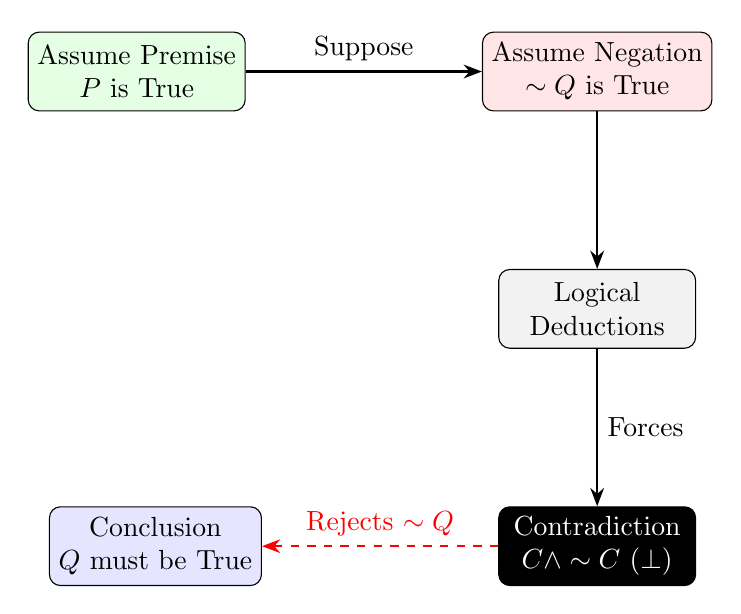
\begin{tikzpicture}[
    node distance=2cm and 3cm,
    box/.style={draw, rectangle, rounded corners, minimum width=2.5cm, minimum height=1cm, align=center, fill=gray!10},
    arrow/.style={->, >=Stealth, thick}
]

% Nodes
\node[box, fill=green!10] (P) {Assume Premise\\$P$ is True};
\node[box, fill=red!10, right=of P] (notQ) {Assume Negation\\$\sim Q$ is True};
\node[box, below=of notQ] (deduce) {Logical\\Deductions};
\node[box, fill=black, text=white, below=of deduce] (bot) {Contradiction\\$C \land \sim C$ ($\bot$)};
\node[box, fill=blue!10, left=of bot] (Q) {Conclusion\\$Q$ must be True};

% Arrows
\draw[arrow] (P) -- (notQ) node[midway, above] {Suppose};
\draw[arrow] (notQ) -- (deduce);
\draw[arrow] (deduce) -- (bot) node[midway, right] {Forces};
\draw[arrow, dashed, red] (bot) -- (Q) node[midway, above] {Rejects $\sim Q$};

\end{tikzpicture}
\end{center}

\subsection{Heuristics \& ``Cheats''}
\begin{itemize}
    \item \textbf{When to use Contradiction:} Use it when the conclusion is a \textit{negative} statement (e.g., ``$x$ is irrational'' meaning ``$x$ is NOT rational'', or ``there is NO largest number''). It is easier to assume the positive existence of something and break it.
    \item \textbf{The ``Divide by 2'' Trick:} When dealing with ``smallest positive'' or ``largest negative'' in dense sets ($\Q, \R$), dividing the assumed extremum by $2$ is the standard cheat code to find a number closer to zero.
\end{itemize}

\subsection{Pitfalls \& Fallacies}
\begin{itemize}
    \item \textbf{Proof by Example:} Providing one example where $\forall x, P(x)$ works does NOT prove the statement. However, providing one counterexample DOES disprove it.
    \item \textbf{Incorrect Negation:} A common trap is negating $P \implies Q$ as $\sim P \implies \sim Q$. The correct negation is $P \land \sim Q$.
\end{itemize}

\newpage
% ==========================================
% PART 5: Conceptual Synthesis
% ==========================================
\section{Part 5: Conceptual Synthesis and The ``Big Picture''}

\subsection{A) Thematic Connections}
The central theme of this chapter is \textbf{Logical Boundary Testing}. Mathematics is not just about computing values; it is about defining the absolute limits of structures. Counterexamples test the boundaries of universal claims, acting as the ``quality assurance'' of mathematics. Proof by contradiction tests the boundaries of logical consistency. By deliberately stepping outside the bounds of truth (assuming $\sim R$), we observe the structural collapse of the mathematical universe (a contradiction), thereby confirming the necessity of the boundary.

\subsection{B) Forward and Backward Links}
\begin{itemize}
    \item \textbf{Backward Links:} This chapter relies heavily on the Direct Proof techniques established in earlier chapters. To derive a contradiction, one must execute a flawless chain of direct deductions from the false premise.
    \item \textbf{Forward Links:} Proof by contradiction is the bedrock of advanced abstract mathematics. In \textbf{Measure Theory}, proving that non-measurable sets exist (like the Vitali set) relies entirely on assuming they are measurable and deriving a contradiction regarding translation invariance and countable additivity. In \textbf{Topology}, proving a space is compact often involves assuming an open cover has no finite subcover and deriving a contradiction.
\end{itemize}

\newpage
% ==========================================
% PART 6: Abstract Real-World Modeling
% ==========================================
\section{Part 6: Abstract Real-World Modeling (AI, ML, \& Quant Finance)}

\subsection{A) Concrete Scenarios}
\begin{enumerate}
    \item \textbf{Quantitative Finance (No-Arbitrage Pricing):} The entire foundation of derivative pricing (Black-Scholes, Martingale Pricing) relies on the assumption of a ``No-Arbitrage'' market. The Fundamental Theorem of Asset Pricing is often proven using contradiction: Assume an arbitrage opportunity exists, construct a self-financing portfolio that yields riskless profit, and contradict the existence of an Equivalent Martingale Measure ($\mathbb{Q}$).
    \item \textbf{Machine Learning (PAC Learning Lower Bounds):} In Statistical Learning Theory, we often want to prove that a hypothesis class $\mathcal{H}$ with infinite VC-dimension cannot be Probably Approximately Correct (PAC) learned. We assume, to the contrary, that a learning algorithm exists, and derive a contradiction by showing it must fail on a specific adversarial data distribution.
\end{enumerate}

\subsection{B) Model Problem Setup: Arbitrage Pricing Theory}
Let us formalize the No-Arbitrage condition using proof by contradiction.

\textbf{Definitions:}
Let $(\Omega, \F, \Prob)$ be a probability space representing all possible market states.
Let $S_t$ be the price of a risky asset at time $t \in \{0, 1\}$, where $S_0$ is a known constant and $S_1$ is an $\F$-measurable random variable.
Let $B_t$ be a risk-free bond with $B_0 = 1$ and $B_1 = 1 + r$, where $r > 0$ is the risk-free rate.
A \textit{trading strategy} is a vector $(x, y) \in \R^2$ representing the units of bonds and stocks held.
The value of the portfolio at time $t$ is $V_t = xB_t + yS_t$.

\textbf{Definition of Arbitrage:}
An arbitrage is a strategy $(x, y)$ such that:
1. $V_0 = 0$ (Zero initial cost)
2. $\Prob(V_1 \ge 0) = 1$ (No risk of loss)
3. $\Prob(V_1 > 0) > 0$ (Positive probability of strict profit)

\textbf{Theorem:} If there exists a risk-neutral probability measure $\mathbb{Q}$ equivalent to $\Prob$ (meaning $\Prob(A)=0 \iff \mathbb{Q}(A)=0$) such that $S_0 = \E_{\mathbb{Q}}\left[\frac{S_1}{1+r}\right]$, then the market contains no arbitrage.

\begin{proof}[Proof (By Contradiction)]
Assume, to the contrary, that such a measure $\mathbb{Q}$ exists, AND an arbitrage strategy $(x, y)$ exists.
Since $(x, y)$ is an arbitrage, $V_0 = x(1) + yS_0 = 0$.
By the martingale property under $\mathbb{Q}$:
\begin{align*}
\E_{\mathbb{Q}}\left[\frac{V_1}{1+r}\right] &= \E_{\mathbb{Q}}\left[\frac{x(1+r) + yS_1}{1+r}\right] \\
&= x + y\E_{\mathbb{Q}}\left[\frac{S_1}{1+r}\right] \\
&= x + yS_0 \\
&= V_0 = 0
\end{align*}
So, $\E_{\mathbb{Q}}[V_1] = 0$.
However, by the definition of arbitrage, $V_1 \ge 0$ almost surely under $\Prob$. Since $\mathbb{Q}$ is equivalent to $\Prob$, $V_1 \ge 0$ almost surely under $\mathbb{Q}$.
Furthermore, $\Prob(V_1 > 0) > 0 \implies \mathbb{Q}(V_1 > 0) > 0$.
The expectation of a non-negative random variable that is strictly positive with non-zero probability must be strictly positive.
Therefore, $\E_{\mathbb{Q}}[V_1] > 0$.
We have derived $\E_{\mathbb{Q}}[V_1] = 0$ and $\E_{\mathbb{Q}}[V_1] > 0$. This is a contradiction ($0 > 0$).
Thus, no arbitrage can exist.
\end{proof}

\newpage
% ==========================================
% PART 7: Common Variations and Untested Concepts
% ==========================================
\section{Part 7: Common Variations and Untested Concepts}

A standard university curriculum in abstract mathematics covers advanced variations of proof by contradiction not present in the provided homework. The most prominent is \textbf{Fermat's Method of Infinite Descent}.

\subsection{Infinite Descent}
Infinite descent is a specific type of proof by contradiction used to show that a property cannot hold for any positive integers. You assume a solution exists, and then prove that if a solution exists, a strictly smaller positive integer solution must also exist. This creates an infinite strictly decreasing sequence of positive integers, which violates the Well-Ordering Principle of $\N$.

\textbf{Theorem:} $\sqrt{2}$ is irrational. (Proven via Infinite Descent).
\begin{proof}
Assume, to the contrary, that $\sqrt{2}$ is rational. Then there exist positive integers $p, q$ such that $\sqrt{2} = \frac{p}{q}$.
This implies $2 = \frac{p^2}{q^2}$, so $p^2 = 2q^2$.
Since $p^2$ is even, $p$ must be even. Let $p = 2p_1$ for some positive integer $p_1 < p$.
Substitute $p$ into the equation:
\[ (2p_1)^2 = 2q^2 \implies 4p_1^2 = 2q^2 \implies q^2 = 2p_1^2 \]
This implies $q^2$ is even, so $q$ must be even. Let $q = 2q_1$ for some positive integer $q_1 < q$.
We now have a new pair of positive integers $(p_1, q_1)$ such that $p_1^2 = 2q_1^2$, meaning $\sqrt{2} = \frac{p_1}{q_1}$.
By repeating this process, we can generate an infinite sequence of strictly decreasing positive integers:
\[ p > p_1 > p_2 > p_3 > \dots > 0 \]
This contradicts the Well-Ordering Principle of the natural numbers (every non-empty subset of $\N$ must have a least element; an infinite strictly decreasing sequence cannot exist in $\N$).
Therefore, $\sqrt{2}$ is irrational.
\end{proof}

\newpage
% ==========================================
% PART 8: Advanced Diagnostic Testing
% ==========================================
\section{Part 8: Advanced Diagnostic Testing: ``Find the Flaw''}

Below are five proofs that contain a subtle, critical logical flaw. Your task as the grader is to identify the error.

\subsection{Flawed Proofs}

\textbf{Problem 1:} Prove that all positive integers are equal.
\begin{proof}
We prove by contradiction. Assume there exist positive integers that are not equal. Let $S$ be the set of all pairs of positive integers $(a, b)$ such that $a \neq b$. By the Well-Ordering Principle, there exists a pair in $S$ with the minimum maximum value. Let this pair be $(x, y)$, and let $M = \max(x, y)$.
Consider the pair $(x-1, y-1)$. Since $x \neq y$, it follows that $x-1 \neq y-1$. Thus $(x-1, y-1) \in S$.
The maximum of this new pair is $\max(x-1, y-1) = M - 1$.
Since $M - 1 < M$, we have found a pair in $S$ with a smaller maximum. This contradicts the assumption that $(x, y)$ had the minimum maximum.
Therefore, no such pair exists, and all positive integers are equal.
\end{proof}

\textbf{Problem 2:} Prove that $\sqrt{4}$ is irrational.
\begin{proof}
Assume, to the contrary, that $\sqrt{4}$ is rational. Then $\sqrt{4} = \frac{p}{q}$ where $p, q \in \Z$, $q \neq 0$, and the fraction is in lowest terms (i.e., $p$ and $q$ share no common factors).
Squaring both sides gives $4 = \frac{p^2}{q^2}$, so $p^2 = 4q^2 = 2(2q^2)$.
Since $p^2$ is a multiple of $2$, $p^2$ is even, which implies $p$ is even. Let $p = 2k$.
Substitute this back: $(2k)^2 = 4q^2 \implies 4k^2 = 4q^2 \implies k^2 = q^2$.
Since $k^2 = q^2$, and $p = 2k$, we have $p^2 = 4k^2$.
Notice that $p$ is even. Since $k^2 = q^2$, if $k$ is even, $q$ is even. If $q$ is even, then both $p$ and $q$ are divisible by $2$. This contradicts the assumption that $\frac{p}{q}$ is in lowest terms.
Therefore, $\sqrt{4}$ is irrational.
\end{proof}

\textbf{Problem 3:} Prove that $1 = 2$.
\begin{proof}
Assume, to the contrary, that $1 \neq 2$.
Let $a = b = 1$.
Multiply both sides by $a$: $a^2 = ab$.
Subtract $b^2$ from both sides: $a^2 - b^2 = ab - b^2$.
Factor both sides: $(a-b)(a+b) = b(a-b)$.
Divide both sides by $(a-b)$: $a + b = b$.
Substitute $a = 1, b = 1$: $1 + 1 = 1 \implies 2 = 1$.
This contradicts our assumption that $1 \neq 2$. Therefore, $1 = 2$.
\end{proof}

\textbf{Problem 4:} Prove that the function $f(x) = \frac{1}{x}$ has a root in the interval $[-1, 1]$.
\begin{proof}
Assume, to the contrary, that $f(x)$ has no root in $[-1, 1]$.
We evaluate the function at the endpoints of the interval:
$f(-1) = \frac{1}{-1} = -1$.
$f(1) = \frac{1}{1} = 1$.
Since $f(-1) < 0$ and $f(1) > 0$, by the Intermediate Value Theorem, there must exist some $c \in (-1, 1)$ such that $f(c) = 0$.
This means $f(x)$ does have a root, which contradicts our assumption.
Therefore, $f(x)$ has a root in $[-1, 1]$.
\end{proof}

\textbf{Problem 5:} Prove that for any two events $A$ and $B$ in a probability space, if $\Prob(A) > 0$ and $\Prob(B) > 0$, then $\Prob(A \cap B) > 0$.
\begin{proof}
Assume, to the contrary, that $\Prob(A \cap B) = 0$.
By the definition of conditional probability, $\Prob(A \mid B) = \frac{\Prob(A \cap B)}{\Prob(B)}$.
Substituting our assumption, $\Prob(A \mid B) = \frac{0}{\Prob(B)} = 0$.
However, since $\Prob(A) > 0$ and $\Prob(B) > 0$, the events must have some probability of occurring. Since the probability of $A$ occurring given $B$ is $0$, this implies $A$ and $B$ are independent, so $\Prob(A \cap B) = \Prob(A)\Prob(B)$.
Since $\Prob(A) > 0$ and $\Prob(B) > 0$, their product $\Prob(A)\Prob(B) > 0$.
Thus, $\Prob(A \cap B) > 0$. This contradicts our assumption that $\Prob(A \cap B) = 0$.
Therefore, $\Prob(A \cap B) > 0$.
\end{proof}

\newpage
\subsection{Solution Key: The Flaws Revealed}

\textbf{Resolution to Problem 1:}
\textit{The Flaw:} The proof assumes that if $(x, y)$ are positive integers, then $(x-1, y-1)$ are also positive integers. This is false if $x=1$ or $y=1$. If $x=1$, then $x-1=0$, which is not a positive integer, meaning $(x-1, y-1) \notin S$. The descent fails at the base case.

\textbf{Resolution to Problem 2:}
\textit{The Flaw:} The logical deduction "if $k$ is even, $q$ is even" is a conditional statement that is never proven to be triggered. The proof establishes $k^2 = q^2$, but it never proves that $k$ \textit{must} be even. In reality, for $\sqrt{4} = 2/1$, $p=2, q=1$, so $k=1$. Since $k$ is odd, $q$ is odd, and they share no common factors. The contradiction is fabricated by an unproven "if".

\textbf{Resolution to Problem 3:}
\textit{The Flaw:} The proof divides both sides by $(a-b)$. Since $a = b = 1$, $a - b = 0$. Division by zero is undefined and violates the field axioms of real numbers. Any logical deduction following a division by zero is invalid (Principle of Explosion).

\textbf{Resolution to Problem 4:}
\textit{The Flaw:} The Intermediate Value Theorem (IVT) strictly requires the function $f(x)$ to be \textit{continuous} on the closed interval $[a, b]$. The function $f(x) = \frac{1}{x}$ has an infinite discontinuity at $x = 0$, which lies within $[-1, 1]$. Therefore, the IVT cannot be applied, and the contradiction is invalid.

\textbf{Resolution to Problem 5:}
\textit{The Flaw:} The proof falsely claims that $\Prob(A \mid B) = 0$ implies $A$ and $B$ are independent. Independence requires $\Prob(A \cap B) = \Prob(A)\Prob(B)$. If $\Prob(A \mid B) = 0$, it means $A$ and $B$ are mutually exclusive (disjoint up to a null set), not independent. The substitution $\Prob(A \cap B) = \Prob(A)\Prob(B)$ is completely unjustified.

\end{document}